\begin{figure}[htbp]
\centering
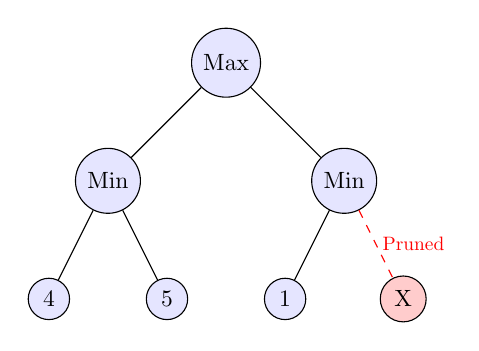
\begin{tikzpicture}[
    level distance=1.5cm,
    level 1/.style={sibling distance=3cm},
    level 2/.style={sibling distance=1.5cm},
    node/.style={circle, draw, minimum size=1.5em, fill=blue!10, scale=0.85},
    pruned/.style={circle, draw, minimum size=1.5em, fill=red!20, scale=0.85},
    arrow/.style={draw, -latex', thick}
]
    \node[node] (root) {Max}
        child {node[node] {Min}
            child {node[node] {4}}
            child {node[node] {5}}
        }
        child {node[node] {Min}
            child {node[node] {1}}
            child {node[pruned] {X}
                edge from parent [dashed, red]
                node[right, scale=0.7] {Pruned}
            }
        };
\end{tikzpicture}
\caption[Conceptual Alpha-Beta Pruning Search Tree]{Conceptual Alpha-Beta Pruning Search Tree with an indicated search cutoff.}
\label{fig:alpha_beta_tree}
\end{figure}
% Source Material: Standard foundational computer science illustration
